%% ============================================================================
\section{Lecture 8: Convective Heat Transport, Boundary Layers, and Clouds}
\label{sec:lec08}
%% ============================================================================
\date{04/06/2026}

\begin{center}
    \textit{Lecture date: 04/06/2026}
\end{center}

The previous lecture derived the local instability criterion for a stratified
fluid: a parcel displaced rapidly enough to remain adiabatic is unstable when
the environmental entropy decreases upward. This lecture uses that criterion
as a working approximation method. Instead of solving the full turbulent flow,
we ask which balances determine the heat flux, the typical convective velocity,
the thickness of the remaining diffusive boundary layers, and the visible
onset of moist atmospheric convection.

%%----------------------------------------------------------------------------
\subsection{From Instability Criterion to Transport Estimate}
\label{sec:lec08:instability-to-transport}
%%----------------------------------------------------------------------------

\subsubsection*{Physical Motivation}
The condition $\Gamma>\Gamma_{\rm ad}$ says that convection starts, but an
order-of-magnitude model must also say what convection does after it starts.
The key physical idea is self-regulation. If the background is strongly
superadiabatic, rising warm parcels and sinking cold parcels carry a large
heat flux; that heat flux reduces the temperature contrast that drove the
motion. If the background is subadiabatic, vertical motions are restored and
the layer transports heat mainly by diffusion or radiation. Efficient
convection therefore tends to keep the bulk fluid close to marginal stability.

\dfn[def:lec08:superadiabatic-gradient]{Superadiabatic Excess}{
Let
\[
    \Gamma\equiv-\frac{dT}{dz},
    \qquad
    \Gamma_{\rm ad}\equiv\frac{g}{c_p}.
\]
The superadiabatic temperature drop across a layer of height $H$ is
\[
    \Delta T_{\rm ex}\equiv
    \left(\Gamma-\Gamma_{\rm ad}\right)H .
\]
Only this excess, not the full temperature drop, gives buoyant acceleration
relative to a neutrally stratified adiabatic background.
}

\subsubsection*{Mathematical Setup}
Let $U$ be the typical convective velocity, $H$ the layer thickness, $\alpha$
the thermal expansion coefficient, and $\Delta T_{\rm ex}$ the temperature
excess of a parcel relative to the neutral adiabatic profile. At fixed
pressure,
\begin{equation}
    \frac{\Delta\rho}{\rho}
    \simeq
    -\alpha\Delta T_{\rm ex}.
    \label{eq:lec08:density-contrast}
\end{equation}
The buoyant acceleration is therefore
\begin{equation}
    a_{\rm buoy}
    \sim
    g\alpha\Delta T_{\rm ex}.
    \label{eq:lec08:buoyant-acceleration}
\end{equation}
If a parcel is accelerated over a distance of order $H$, the work per unit
mass is $a_{\rm buoy}H$. Equating that to the kinetic energy per unit mass
$U^2$ gives
\begin{equation}
    U^2\sim g\alpha\Delta T_{\rm ex}H.
    \label{eq:lec08:velocity-energy-balance}
\end{equation}
Thus
\begin{equation}
    \boxed{
    U\sim\left(g\alpha\Delta T_{\rm ex}H\right)^{1/2}.
    }
    \label{eq:lec08:convective-velocity}
\end{equation}
\textit{Significance:} The velocity is not an externally imposed scale; it is
the speed required for buoyancy to convert the available potential energy of
the unstable stratification into motion.

The same estimate can be written as a buoyancy time:
\begin{equation}
    \boxed{
    \tau_{\rm buoy}\sim\frac{H}{U}
    \sim
    \left(\frac{H}{g\alpha\Delta T_{\rm ex}}\right)^{1/2}.
    }
    \label{eq:lec08:buoyancy-time}
\end{equation}
\textit{Significance:} A layer is dynamically convective only if buoyancy acts
before thermal diffusion erases the parcel's temperature anomaly.

%%----------------------------------------------------------------------------
\subsection{Convective Heat Flux as a Mixing Estimate}
\label{sec:lec08:convective-flux}
%%----------------------------------------------------------------------------

\subsubsection*{Conceptual Background}
Microscopic conduction transports heat because molecules carry thermal energy
over a mean free path. Turbulent convection is the same approximation at a
larger scale: eddies carry entropy and temperature anomalies over a mixing
length before they lose their identity. The details of the turbulent cascade
are complicated, but the flux estimate only needs three ingredients:
\begin{itemize}
    \item the heat capacity per unit volume, $\rho c_p$;
    \item the temperature anomaly being carried, $\Delta T_{\rm ex}$;
    \item the speed with which the anomaly crosses the layer, $U$.
\end{itemize}

\subsubsection*{Mathematical Setup}
The thermal energy per unit volume associated with a temperature anomaly
$\Delta T_{\rm ex}$ is of order $\rho c_p\Delta T_{\rm ex}$. A velocity $U$
carries that energy through a unit area per unit time, so
\begin{equation}
    F_{\rm conv}
    \sim
    \rho c_p U\Delta T_{\rm ex}.
    \label{eq:lec08:convective-flux-basic}
\end{equation}
Substituting Eq.~\eqref{eq:lec08:convective-velocity},
\begin{equation}
    \boxed{
    F_{\rm conv}
    \sim
    \rho c_p
    \left(g\alpha H\right)^{1/2}
    \left(\Delta T_{\rm ex}\right)^{3/2}.
    }
    \label{eq:lec08:convective-flux}
\end{equation}
\textit{Significance:} Convective flux grows faster than linearly with the
superadiabatic excess, so a very small departure from marginal stability can
carry a large heat flux when convection is efficient.

If the required outward heat flux $F$ is known, the estimate can be inverted:
\begin{align}
    F
    &\sim
    \rho c_p
    \left(g\alpha H\right)^{1/2}
    \left(\Delta T_{\rm ex}\right)^{3/2},
    \label{eq:lec08:flux-inversion-step}\\
    \Delta T_{\rm ex}
    &\sim
    \left[
        \frac{F}{\rho c_p\left(g\alpha H\right)^{1/2}}
    \right]^{2/3}.
    \label{eq:lec08:superadiabatic-excess-from-flux}
\end{align}
Thus
\begin{equation}
    \boxed{
    \frac{\Delta T_{\rm ex}}{H}
    \sim
    \left[
        \frac{F^2}{\rho^2c_p^2g\alpha H^4}
    \right]^{1/3}.
    }
    \label{eq:lec08:superadiabatic-gradient-from-flux}
\end{equation}
\textit{Significance:} A measured or imposed flux fixes the small excess
gradient needed above the adiabatic gradient; this is why strongly convective
regions are often nearly, but not exactly, adiabatic.

\nt{This is a scaling closure, not a precise turbulence theory. Numerical
coefficients, entrainment, compressibility, and detailed geometry are hidden in
order-unity factors. The useful approximation is the dependence on $F$, $g$,
$\alpha$, $H$, $\rho$, and $c_p$.}

%%----------------------------------------------------------------------------
\subsection{Boundary Layers in Efficient Convection}
\label{sec:lec08:convective-boundary-layers}
%%----------------------------------------------------------------------------

\subsubsection*{Physical Motivation}
When convection is efficient, the bulk layer mixes entropy rapidly and becomes
almost adiabatic. But a solid boundary cannot be crossed by the fluid, and
near the boundary the vertical velocity must vanish. Heat must then cross a
thin boundary layer by conduction before it enters the well-mixed convective
interior. This is the same approximation logic used in diffusion problems:
identify the region where the neglected process becomes dominant.

\begin{figure}[ht]
    \centering
    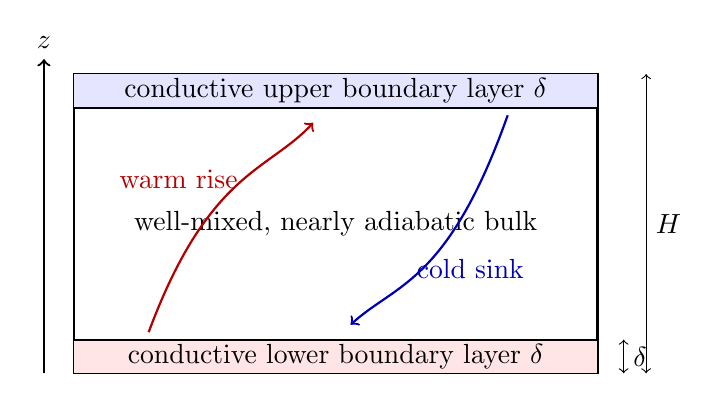
\begin{tikzpicture}[scale=0.95]
        \draw[thick] (0,0) rectangle (7,4);
        \fill[red!10] (0,0) rectangle (7,0.45);
        \fill[blue!10] (0,3.55) rectangle (7,4);
        \draw[thick,->] (-0.4,0) -- (-0.4,4.2) node[above] {$z$};
        \draw[thick] (0,0.45) -- (7,0.45);
        \draw[thick] (0,3.55) -- (7,3.55);
        \node at (3.5,0.22) {conductive lower boundary layer $\delta$};
        \node at (3.5,3.78) {conductive upper boundary layer $\delta$};
        \node at (3.5,2.0) {well-mixed, nearly adiabatic bulk};
        \draw[->,red!70!black,thick] (1.0,0.55) .. controls (1.8,2.7) and (2.6,2.7) .. (3.2,3.35);
        \draw[->,blue!70!black,thick] (5.8,3.45) .. controls (5.0,1.2) and (4.3,1.2) .. (3.7,0.65);
        \node[red!70!black] at (1.4,2.6) {warm rise};
        \node[blue!70!black] at (5.3,1.4) {cold sink};
        \draw[<->] (7.35,0) -- (7.35,0.45) node[midway,right] {$\delta$};
        \draw[<->] (7.65,0) -- (7.65,4) node[midway,right] {$H$};
    \end{tikzpicture}
    \caption{Efficient convection leaves most of the layer close to an
    adiabatic, well-mixed state. The imposed temperature drop is concentrated
    in thin conductive boundary layers of thickness $\delta$.}
    \label{fig:lec08:convective-boundary-layer}
\end{figure}

\subsubsection*{Mathematical Setup}
Let $\chi$ be the thermal diffusivity. A plume that moves with speed $U$ crosses
the layer in the turnover time
\begin{equation}
    \tau_{\rm turn}\sim\frac{H}{U}.
    \label{eq:lec08:turnover-time}
\end{equation}
Thermal diffusion penetrates a distance $\delta$ in the same time if
\begin{equation}
    \delta^2\sim \chi\tau_{\rm turn}.
    \label{eq:lec08:boundary-layer-diffusion-step}
\end{equation}
Therefore
\begin{equation}
    \boxed{
    \delta\sim\left(\frac{\chi H}{U}\right)^{1/2}.
    }
    \label{eq:lec08:thermal-boundary-layer}
\end{equation}
\textit{Significance:} Faster convection makes the conductive boundary layer
thinner because heat has less time to diffuse sideways or vertically before the
fluid is replaced.

The conductive heat flux through a boundary layer is
\begin{equation}
    F_{\rm cond}
    \sim
    \rho c_p\chi\frac{\Delta T_{\rm bl}}{\delta},
    \label{eq:lec08:boundary-layer-flux}
\end{equation}
where $\Delta T_{\rm bl}$ is the temperature drop across the boundary layer.
The same total flux must pass through the boundary layer and the convective
bulk, so the boundary layer often controls the total thermal resistance.

\dfn[def:lec08:nusselt-number]{Nusselt Number}{
The Nusselt number compares total heat transport to the heat transport that
would occur by pure conduction across the full layer:
\[
    \mathrm{Nu}\equiv
    \frac{F}{\rho c_p\chi\,\Delta T/H}.
\]
Equivalently, if the total drop $\Delta T$ is mainly across two comparable
boundary layers, then $\mathrm{Nu}\sim H/\delta$ up to factors of order unity.
}

Using Eq.~\eqref{eq:lec08:thermal-boundary-layer},
\begin{equation}
    \boxed{
    \mathrm{Nu}\sim\frac{H}{\delta}
    \sim
    \left(\frac{UH}{\chi}\right)^{1/2}.
    }
    \label{eq:lec08:nusselt-peclet}
\end{equation}
\textit{Significance:} Heat transport is enhanced above conduction when the
thermal Peclet number $UH/\chi$ is large, because advection replaces slow
molecular diffusion across most of the layer.

%%----------------------------------------------------------------------------
\subsection{Dimensionless View: Rayleigh, Prandtl, Peclet, and Reynolds}
\label{sec:lec08:dimensionless-view}
%%----------------------------------------------------------------------------

\subsubsection*{Conceptual Background}
The lecture repeatedly uses the same approximation strategy: first list the
physical effects, then form dimensionless ratios that compare their
timescales. For convection the effects are buoyancy, viscous diffusion of
momentum, and thermal diffusion of heat.

The relevant definitions are
\begin{equation}
    \mathrm{Re}\equiv\frac{UH}{\nu},
    \qquad
    \mathrm{Pe}\equiv\frac{UH}{\chi},
    \qquad
    \mathrm{Pr}\equiv\frac{\nu}{\chi}.
    \label{eq:lec08:re-pe-pr-definitions}
\end{equation}
Therefore
\begin{equation}
    \boxed{
    \mathrm{Pe}=\mathrm{Re}\,\mathrm{Pr}.
    }
    \label{eq:lec08:peclet-re-pr}
\end{equation}
\textit{Significance:} A flow can be dynamically turbulent and still thermally
diffusive if $\mathrm{Re}$ is large but $\mathrm{Pe}$ is not; momentum and heat
need not be transported with the same efficiency.

The Rayleigh number is
\begin{equation}
    \mathrm{Ra}
    =
    \frac{g\alpha\Delta T_{\rm ex}H^3}{\nu\chi}.
    \label{eq:lec08:rayleigh-definition}
\end{equation}
Using $U^2\sim g\alpha\Delta T_{\rm ex}H$,
\begin{align}
    \mathrm{Ra}
    &\sim
    \frac{U^2H^2}{\nu\chi}
    =
    \left(\frac{UH}{\nu}\right)
    \left(\frac{UH}{\chi}\right)  \nonumber\\
    &=
    \mathrm{Re}\,\mathrm{Pe}
    =
    \mathrm{Re}^2\mathrm{Pr}.
    \label{eq:lec08:rayleigh-re-pe}
\end{align}
Thus
\begin{equation}
    \boxed{
    \mathrm{Re}\sim\left(\frac{\mathrm{Ra}}{\mathrm{Pr}}\right)^{1/2},
    \qquad
    \mathrm{Pe}\sim\left(\mathrm{Ra}\,\mathrm{Pr}\right)^{1/2}.
    }
    \label{eq:lec08:re-pe-from-ra-pr}
\end{equation}
\textit{Significance:} Once buoyancy sets the velocity, $\mathrm{Ra}$ and
$\mathrm{Pr}$ determine whether the resulting convective motion is inertial,
viscous, thermally diffusive, or thermally advective.

%%----------------------------------------------------------------------------
\subsection{Moist Atmospheric Convection and Cloud Formation}
\label{sec:lec08:moist-convection-clouds}
%%----------------------------------------------------------------------------

\subsubsection*{Physical Motivation}
Clouds are a visible marker of the same parcel argument. A surface-heated air
parcel rises, expands because the ambient pressure is lower, and cools
approximately adiabatically. If it contains water vapor, the saturation vapor
pressure decreases rapidly as the parcel cools. Once the actual vapor pressure
reaches saturation, condensation begins. Latent heat release then changes the
adiabatic relation and makes the effective lapse rate smaller than the dry
value.

\begin{figure}[ht]
    \centering
    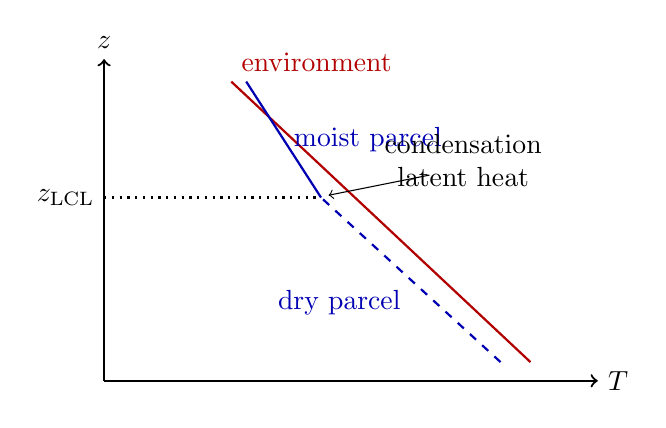
\begin{tikzpicture}[scale=0.95]
        \draw[thick,->] (0,0) -- (0,4.3) node[above] {$z$};
        \draw[thick,->] (0,0) -- (6.6,0) node[right] {$T$};
        \draw[red!70!black,thick] (5.7,0.25) -- (1.7,4.0)
            node[above right] {environment};
        \draw[blue!70!black,thick,dashed] (5.3,0.25) -- (2.9,2.45)
            node[midway,below left] {dry parcel};
        \draw[blue!70!black,thick] (2.9,2.45) -- (1.9,4.0)
            node[midway,right] {moist parcel};
        \draw[dotted,thick] (0,2.45) -- (2.9,2.45);
        \node[left] at (0,2.45) {$z_{\rm LCL}$};
        \node[align=center] at (4.8,2.95) {condensation\\latent heat};
        \draw[->] (4.35,2.75) -- (3.0,2.48);
    \end{tikzpicture}
    \caption{A rising parcel cools along a dry adiabat until it reaches the
    lifting condensation level $z_{\rm LCL}$. Above that height, condensation
    releases latent heat and the parcel follows a shallower moist adiabat.}
    \label{fig:lec08:moist-parcel-cloud}
\end{figure}

\subsubsection*{Mathematical Setup}
For a dry ideal-gas parcel,
\begin{equation}
    \left(\frac{dT}{dz}\right)_{\rm dry}
    =
    -\frac{g}{c_p}.
    \label{eq:lec08:dry-lapse}
\end{equation}
If a mass fraction $dq_s$ of vapor condenses per unit mass of dry air and $L$
is the latent heat per unit mass, the first-law balance per unit mass becomes
\begin{equation}
    c_p\,dT-\frac{1}{\rho}\,dP=-L\,dq_s.
    \label{eq:lec08:moist-first-law}
\end{equation}
The left-hand side is the dry adiabatic cooling term. The right-hand side is
negative when saturation mixing ratio decreases upward, $dq_s<0$, so
$-L\,dq_s>0$ supplies heat to the parcel. Therefore the magnitude of the
temperature decrease with height is reduced:
\begin{equation}
    \boxed{
    \Gamma_{\rm moist}
    \equiv
    -\left(\frac{dT}{dz}\right)_{\rm moist}
    <
    \Gamma_{\rm dry}
    =
    \frac{g}{c_p}.
    }
    \label{eq:lec08:moist-lapse-inequality}
\end{equation}
\textit{Significance:} Moist air can remain buoyant in an atmosphere that
would be stable for a dry parcel, because condensation returns latent heat to
the rising parcel.

The approximate lifting condensation level follows from comparing the initial
temperature $T_0$ to the dew-point temperature $T_d$. If both are expressed in
degrees Celsius and the parcel cools at roughly
$\Gamma_{\rm dry}\simeq 10\,\si{K\,km^{-1}}$ before condensation, while the
dew point changes more slowly, a useful estimate is
\begin{equation}
    \boxed{
    z_{\rm LCL}
    \sim
    \frac{T_0-T_d}{\Gamma_{\rm dry}}
    \simeq
    100\,\si{m}\times
    \left(\frac{T_0-T_d}{1\,\si{K}}\right).
    }
    \label{eq:lec08:lcl-estimate}
\end{equation}
\textit{Significance:} The cloud base height is controlled mainly by how close
surface air is to saturation: humid air has a small $T_0-T_d$ and forms clouds
after a short rise.

\nt{Cumulus clouds indicate localized buoyant plumes that reach saturation.
Cumulonimbus clouds correspond to much deeper, more energetic convection in
which latent heating helps sustain large vertical velocities over many
kilometers.}

%%----------------------------------------------------------------------------
\subsection{Order-of-Magnitude Checklist for Convective Problems}
\label{sec:lec08:oom-checklist}
%%----------------------------------------------------------------------------

\subsubsection*{Motivation}
The approximation-methods goal is not to memorize a single formula, but to
choose a controlled hierarchy of estimates. For a convection problem, a useful
sequence is:
\begin{enumerate}
    \item identify the neutral reference state, usually hydrostatic and
    adiabatic;
    \item estimate the superadiabatic excess $\Delta T_{\rm ex}$, not just the
    total temperature difference;
    \item compare buoyancy, viscous diffusion, and thermal diffusion through
    $\mathrm{Ra}$ and $\mathrm{Pr}$;
    \item if convection is efficient, estimate $U$, $F_{\rm conv}$, and the
    residual boundary-layer thickness $\delta$;
    \item for moist air, check saturation because latent heat changes the
    effective lapse rate and therefore the buoyancy.
\end{enumerate}

\clm[clm:lec08:convection-closure]{Practical Convection Closure}{
For order-of-magnitude work, efficient convection is modeled as a nearly
adiabatic bulk plus thin boundary layers. The bulk determines the buoyant
velocity scale, while the boundary layers often determine the total heat flux.
}

The final mental model is therefore a matched approximation: an outer region
that is well mixed and nearly adiabatic, and inner regions near boundaries or
phase-transition levels where diffusion, radiation, or latent heat cannot be
ignored.
